\documentclass[11pt,a4paper, twocolumn]{jsarticle}

\makeatletter

%%% 個人設定 
\usepackage{amsmath,amssymb}
\usepackage{amsthm}
\usepackage{graphicx}

\bibliographystyle{plain}

\newcommand{\R}{\mathbf R}
\newcommand{\N}{\mathbf N}
\newcommand{\Q}{\mathbf Q}
\newcommand{\Z}{\mathbf Z}
\newcommand{\T}{\{0\}^*}
\newcommand{\D}[1]{D^{(#1)}}
\newcommand{\classP}{\mathbf{P}}
\newcommand{\classPSPACE}{\mathbf{PSPACE}}
\newcommand{\classNP}{\mathbf{NP}}
\newcommand{\classPH}{\mathbf{PH}}
\newcommand{\classPP}{\mathbf{PP}}
\newcommand{\classCH}{\mathbf{CH}}
\newcommand{\C}{\mathbf{C}}

\theoremstyle{definition}
\newtheorem{theorem}{定理}[section]
\newtheorem{lemma}[theorem]{補題}
\newtheorem{collorary}[theorem]{系}
\newtheorem{definition}[theorem]{定義}
\newtheorem{hypothesis}[theorem]{仮定}

\renewcommand{\proofname}{\bf 証明} 

%%% \proc != 0 ならば証明などをとばす.
\newcommand{\proc}{1}


%%% 数式中の大文字ギリシャ文字を斜体化
\renewcommand{\Lambda}{\varLambda}
\renewcommand{\Gamma}{\varGamma}

%%% (i), (ii), (iii), (iv)
\def\theenumi{\roman{enumi}}
\def\labelenumi{(\theenumi)}

%%% 数式番号を(章.num) に
\renewcommand{\theequation}{\thesection.\arabic{equation}}
\@addtoreset{equation}{section}

%%% 表番号を 章.num に
\renewcommand{\thetable}{\thesection.\arabic{table}}
\@addtoreset{table}{section}

%%% 図番号を 章.num に
\renewcommand{\thefigure}{\thesection.\arabic{figure}}
\@addtoreset{figure}{section}

%%% align* などで指定した場所だけ数式番号を置く
\newcommand{\taghere}{{
\stepcounter{equation}
\tag{\theequation}
}}

\makeatother

\title{滑らかな常微分方程式の計算量}

\author{%
\hspace*{7zw}% 良い子は真似してはいけません!
太田浩行\thanks{東京大学, \texttt{hota@is.s.u-tokyo.ac.jp}} 
\and
河村彰星\thanks{東京大学}%
\hspace*{7zw}% 良い子は真似してはいけません!
\and
マルチン・ツィーグラー\thanks{Martin Ziegler, ダルムシュタット工科大学}
\and
カルステン・レースニク\thanks{Carsten R\"osnick, ダルムシュタット工科大学}
}
%\和暦
\date{}

\begin{document}

\maketitle

%%% 以下に,予稿の本文を記述して下さい.

\begin{abstract}
The computational complexity of the solution~$h$ to 
the ordinary differential equation 
$h(0)=0$, $h'(t) = g(t, h(t))$ 
under various assumptions on the function $g$
has been investigated
in hope of understanding the intrinsic hardness of 
solving the equation numerically. 
Kawamura showed in 2010 that the solution~$h$ can be $\classPSPACE$-hard
even if $g$ is assumed to be Lipschitz continuous and polynomial-time computable. 
We place further requirements on the smoothness of $g$ 
and obtain the following results: 
the solution~$h$ is still $\classPSPACE$-hard
if $g$ is assumed to be of class $\classC ^1$; 
for each $k \geq 2$, 
the solution~$h$ is hard for the counting hierarchy 
if $g$ is assumed to be of class $\classC ^k$. 
\end{abstract}


\section{Introduction}

Let $g \colon [0,1] \times \R \to \R$ be continuous 
and consider the differential equation 
\begin{align}
 \label{eq:ode}
 h(0) & = 0, &
 \D h(t) & = g(t,h(t)) \quad t \in [0,1], 
\end{align}
where $\D h$ denotes the derivative of $h$. 
How complex can the solution~$h$ be, 
assuming that $g$ is polynomial-time computable? 
Here, polynomial-time computability 
and other notions of complexity 
are from the field of 
\emph{Computable Analysis}~\cite{weihrauch00:_comput_analy}
and measure how hard it is to 
approximate real functions with specified precision 
(Section~\ref{section: preliminaries}). 

If we put no assumption on $g$ other than being polynomial-time computable, 
the solution~$h$ (which is not unique in general) can be non-computable. 
Table~\ref{table:related} summarizes known results about 
the complexity of $h$ under various assumptions 
(that get stronger as we go down the table). 
In particular, if $g$ is (globally) Lipschitz continuous, 
then the (unique) solution $h$ is known to be 
polynomial-space computable but still can be 
$\classPSPACE$-hard \cite{kawamura2010lipschitz}. 
In this paper, we study the complexity of $h$ 
when we put stronger assumptions about 
the smoothness of $g$. 

\begin{table}
\renewcommand\arraystretch{1.3}
\begin{center}
 \caption{The complexity of the solution $h$ of \eqref{eq:ode}
 assuming $g$ is polynomial-time computable.}
 \label{table:related}
 \begin{tabular}{lll}
  Assumptions & Upper bounds & Lower bounds \\
  \hline
   --- & --- & can be all non-computable \cite{pour1979computable} \\
  $h$ is the unique solution & computable \cite{coddington1955theory}
  & can take arbitrarily long time \cite{ko1983computational,miller1970recursive} \\
  the Lipschitz condition  & polynomial-space \cite{ko1983computational}
      &	can be $\classPSPACE$-hard \cite{kawamura2010lipschitz}\\
  $g$ is of class $\classC ^{(\infty, 1)}$ & polynomial-space 
      & can be $\classPSPACE$-hard (Theorem~\ref{DifferentiableIsPspace}) \\
  \parbox[t]{11em}{$g$ is of class $\classC ^{(\infty, k)}$\\{}(for each constant $k$)}
  & polynomial-space & can be $\classCH$-hard (Theorem~\ref{KTimesIsCH}) \\
  $g$ is analytic
  & polynomial-time \cite{muller1987uniform,ko1988computing} 
  & ---
 \end{tabular}
\end{center}
\end{table}

In numerical analysis, 
knowledge about smoothness of the input function 
(such as being differentiable enough times) 
is often beneficial 
in applying certain algorithms or simplifying their analysis.
However, 
to our knowledge, 
this casual understanding that smoothness is good 
has not been rigorously substantiated 
in terms of computational complexity theory. 
This motivates us to ask whether, 
for our differential equation \eqref{eq:ode}, 
smoothness really reduces the complexity of the solution. 

At the extreme is the case where $g$ is analytic: 
$h$ is then shown to be polynomial-time computable 
(the last row of the table) 
by an argument based on Taylor series. 
Thus our interest is in 
the cases between Lipschitz and analytic 
(the fourth and fifth rows). 
We say that $g$ is of class $\classC ^{(i, j)}$
if the partial derivative $\D ^{(i, j)} g$ 
(often also denoted $\partial ^{i + j} g (t, y) / \partial t ^i \partial y ^j$)
exists and is continuous%
\footnote{%
Another common terminology is to say that $g$ is of class $\classC ^k$
if it is of class $\classC ^{(i,j)}$ 
for all $i$, $j$ with $i + j \leq k$.}; 
it is said to be of class $\classC ^{(\infty, j)}$ if
it is of class $\classC ^{(i, j)}$ for all $i \in \N$. 

\begin{theorem}
 \label{DifferentiableIsPspace}
There is a polynomial-time computable function
$g \colon [0,1] \times [-1,1] \to \R$ 
of class $\classC ^{(\infty, 1)}$ such that
the equation \eqref{eq:ode} has a 
$\classPSPACE$-hard solution $h \colon [0, 1] \to \R$. 
 \end{theorem}

 \begin{theorem}
  \label{KTimesIsCH}
Let $k$ be a positive integer. 
There is a polynomial-time computable function
$g \colon [0,1] \times [-1,1] \to \R$ 
of class $\classC ^{(\infty, k)}$ such that
the equation \eqref{eq:ode} has a 
$\classCH$-hard solution $h \colon [0, 1] \to \R$, 
where $\classCH \subseteq \classPSPACE$ is the 
Counting Hierarchy (see Section~\ref{subsection: counting hierarchy}). 
 \end{theorem}

We said
$g \colon [0,1] \times [-1, 1] \to \R$ instead of 
$g \colon [0,1] \times \R \to \R$, because
the notion of polynomial-time computability of real functions 
is defined in this paper only when the domain is a bounded closed region. 
This notational choice makes
the equation~\eqref{eq:ode} ill-defined 
in case $h$ ever takes a value outside $[-1, 1]$; 
by saying that $h$ is a solution in Theorem~\ref{DifferentiableIsPspace}, 
we are also claiming that 
$h (t) \in [-1, 1]$ for all $t \in [0, 1]$. 
In any case, 
since we are putting stronger assumptions on $g$ than Lipschitz continuity, 
such a solution $h$, if it exists, is unique. 

The questions of whether smoothness of the input function 
reduces the complexity of the output
have been asked for operations other than solving differential equations, 
and the following negative results are known. 
The integral of a polynomial-time computable real function 
can be $\classNumberP$-hard, and this does not change 
by restricting the input to 
$\classC ^\infty$ (infinitely differentiable) functions
\cite[Theorem~5.33]{ko1991complexity}. 
Similarly, the function obtained by maximization 
from a polynomial-time computable real function 
can be $\classNP$-hard, and this is still so
even if the input function is restricted to $\classC ^\infty$ 
\cite[Theorem~3.7]{ko1991complexity}%
\footnote{%
The proof of this fact in \cite[Theorem 3.7]{ko1991complexity}
needs to be fixed by redefining 
\[f(x) = 
\begin{cases}
 u_s & \text{if not } R(s,t), \\
 u_s + 2^{-(p(n)+2n+1)\cdot n} \cdot h_1(2^{p(n)+2n+1} (x - y_{s,t})) & \text{if } R(s,t). 
\end{cases}\]
}. 
(Restricting to analytic inputs 
renders the output polynomial-time computable, 
again because of the argument based on Taylor series.)
In contrast, 
although we have Theorem~\ref{KTimesIsCH} for each $k$, 
we do not know about the complexity of 
$h$ when $g$ is assumed to be infinitely differentiable. 

\subsubsection*{Notation}
Let $\N$, $\Z$, $\Q$, $\R$ denote the set of natural numbers,
integers,
rational numbers and 
real numbers, respectively.

Let $A$ and $B$ be bounded closed intervals in $\R$.
We write $|f| = \sup_{x \in A} f(x)$ for $f \colon A \to \R$.
A function $f \colon A \to \R$ is \emph{of class $\classC^i$}
($i$-times continuously differentiable)
if all the derivatives $\D f, \D^2 f, \dots, \D^i f$ exist and are continuous.

For a differentiable function $g$ of two variables, 
we write $\D _1 g$ and $\D _2 g$ for the derivatives of $g$ 
with respect to the first and the second variable,
respectively.
A function $g \colon A \times B \to \R$ is of \emph{class $\classC^{(i, j)}$}
if for each $n \in \{0, \dots, i\}$ and $m \in \{0, \dots j\}$,
the derivative $\D_1^n \D_2^m g$ exists and is continuous.
A function $g$ is of \emph{class $\classC^{(\infty, j)}$}
if it is of class $\classC^{(i, j)}$ for all $i \in \N$.
When $g$ is of class $\classC^{(i,j)}$,
we write $\D^{(i,j)}g$ for the derivative $\D_1^i \D_2^j g$.

\section{Computational Complexity of Real Functions}
\label{section: preliminaries}

This section reviews the complexity notions 
in Computable Analysis~%
\cite{ko1991complexity,weihrauch00:_comput_analy}. 
We start by fixing an encoding of real numbers 
by string functions.

\begin{definition}
 A function $\phi \colon \{0\} ^* \to \{0, 1\}^*$ is a \emph{name} of a real number $x$ 
 if for all $n \in \N$,
  $\phi(0^n)$ is the binary representation of $\lfloor x \cdot 2^n \rfloor$ or
  $\lceil x \cdot 2^n \rceil$,
 where $\lfloor \cdot \rfloor$ and $\lceil \cdot \rceil$ mean
 rounding down and up to the nearest integer.
 \end{definition}

In effect, a name of a real number $x$ receives $0 ^n$ and 
returns an approximation of $x$ with precision $2 ^{-n}$.

We use \emph{oracle Turing machines} (henceforth just \emph{machines})
to work on these names (Fig.~\ref{fig:model-of-function}).
Let $M$ be a machine and $\phi$ be a function from strings to strings. 
We write $M ^\phi (0 ^n)$ for the output string 
when $M$ is given
$\phi$ as oracle and string $0^n$ as input.
Thus we also regard $M^\phi$ as a function from strings to strings.

\begin{figure}
 \begin{center}
  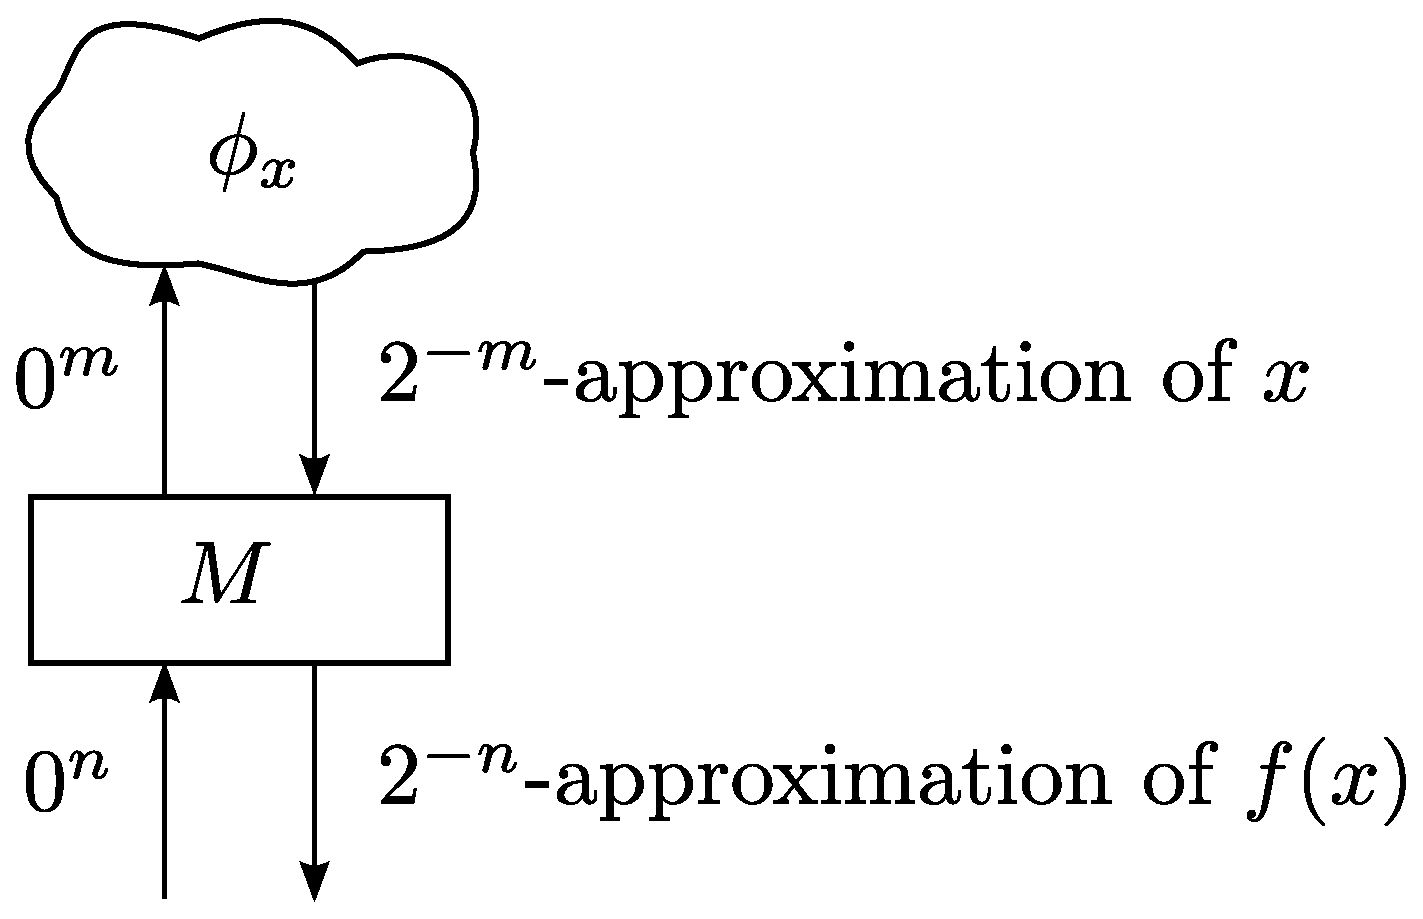
\includegraphics[height=0.17\textheight]{image/model-of-function.eps}
 \end{center}
 \caption{A machine $M$ computing a real function $f$}
 \label{fig:model-of-function}
\end{figure}

\begin{definition}
Let $A$ be a bounded closed interval of\/ $\R$.
A machine $M$ \emph{computes} a real function $f \colon A \to \R$ 
if for any $x \in A$ and any name $\phi_x$ of it,
$M^{\phi_x}$ is a name of $f(x)$.
\end{definition}

Computation of a function $f \colon A \to \R$ on
a two-dimensional bounded closed region $A \subseteq \R ^2$ 
is defined in a similar way using machines with two oracles.
A real function is (\emph{polynomial-time}) \emph{computable} if there exists some machine that computes it (in polynomial time).
Polynomial-time computability of a real function $f$ means that
for any $n \in \N$, 
an approximation of $f(x)$ with error bound $2^{-n}$
is computable in time polynomial in $n$ 
independent of the real number $x$.

By the time the machine outputs the approximation of $f (x)$ of precision~$2 ^{-n}$, 
it knows $x$ only with some precision $2 ^{-m}$.
This implies that all computable real functions are continuous.
If the machine runs in polynomial time,
this $m$ is bounded polynomially in $n$.
This implies \eqref{eq:modulus} in the following lemma, 
which characterizes polynomial-time real functions
by the usual polynomial-time computability of string functions 
without using oracle machines. 

\begin{lemma}
 \label{lem:type1representation}
 A real function is polynomial-time computable if and only if
 there exist a polynomial-time computable function 
 $\phi \colon (\Q \cap [0, 1]) \times \{0\} ^* \to \Q$ and 
 polynomial $p \colon \N \to \N$ such that
 for all $d \in \Q \cap [0,1]$ and $n \in \N$,
 \begin{equation}
  |\phi(d, 0^n) - f(d)| \le 2^{-n},
 \end{equation}
 and for all $x, y \in [0, 1]$, $n \in \N$,
 \begin{equation} 
  |x-y| \le 2^{-p(n)} \Rightarrow |f(x) - f(y)| \le 2^{-n},
   \label{eq:modulus}
 \end{equation}
where each rational number is written
as a fraction whose numerator and denominator
are integers in binary.
\end{lemma}

To talk about hardness, we define reduction. 
A language $L \subseteq \{0, 1\} ^*$ is identified with the function
$L \colon \{0, 1\} ^* \to \{0, 1\}$ such that $L (u) = 1$ when $u \in L$.

\begin{definition} \label{definition: reduction}
 A language $L$ \emph{reduces} to a function $f \colon [0, 1] \to \R$
 if there exists a polynomial-time function $S$ and a polynomial-time oracle Turing machine $M$ (Fig.~\ref{fig:reduction})
 such that for any string $u$, 
  \begin{enumerate}
   \item $S(u, \cdot)$ is a name of a real number $x_u$, and 
   \item $M^\phi(u)$ accepts if and only if $u \in L$ for any name $\phi$ of $f(x_u)$.
  \end{enumerate}
\end{definition}
This reduction may look stronger (and hence the reducibility weaker) than
the one in Kawamura~\cite{kawamura2010lipschitz} 
in that $M$ can make multiple queries adaptively, 
but this makes no difference, 
because the lengths of these queries 
are bounded by a polynomial in $\lvert u \rvert$, 
and the longest query gets all the information that any shorter query gets. 

For a complexity class~$C$, a function $f$ is \emph{$C$-hard}
if all languages in $C$ reduce to $f$.

 \begin{figure}
  \begin{center}
  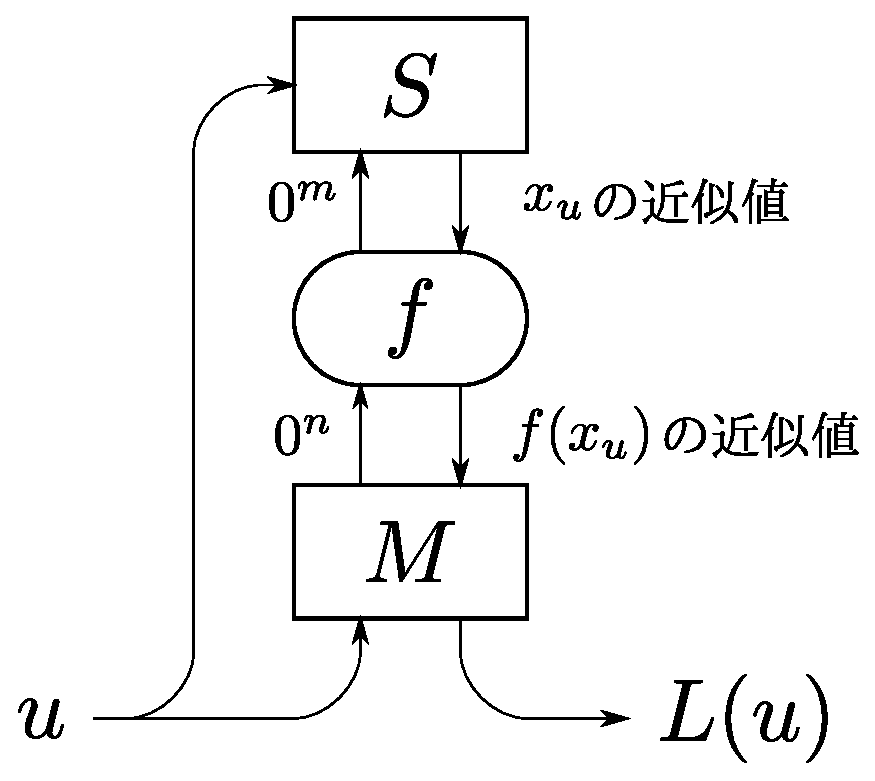
\includegraphics[scale=0.25]{image/reduction.eps}
  \caption{Reduction from a language $L$ to a function $f \colon [0,1] \to \R$}
  \label{fig:reduction}
  \end{center}
 \end{figure}


\section{1回連続微分可能関数と常微分方程式}
\label{section:differentiable}

この節では定理 \ref{DifferentiableIsPspace},
つまり$(\infty, 1)$階連続微分可能な関数の常微分方程式の解は
\PSPACE 困難でありうることを示す.
\ifnum \proc = 1
ただし紙面の都合上, 詳細な証明は省き, 証明の概略を述べるに止める.
\fi

証明の流れとして, まず補題 \ref{WeakFeedback} によりの
$L \in \PSPACE$ を認識する関数族$(G_u)_u, (H_u)_u$ を得る.
そして $(G_u)_u, (H_u)_u$ を模倣する
実関数族 $(g_u)_u, (h_u)_u$ を構成し(補題 \ref{DifferentiableFamily}),
$(g_u)_u, (h_u)_u$ から定理 \ref{DifferentiableIsPspace} で求める $g, h$を構成する.


\subsection{多項式段一様関数族の差分方程式と\PSPACE}


任意の言語 $L \in \PSPACE$ について, 
その差分方程式が $L$ を認識する
多項式段一様な関数族 $(G_u)_u$ が存在すること(補題 \ref{WeakFeedback})は
河村によって示されているがその証明の概略を示す.

\PSPACE 完全な言語である
\textsf{QBF} を認識する $(G_u)_u$ を構成することにより,
任意の $L \in \PSPACE$ を認識する多項式段一様な関数族 $(G_u)_u$ が存在することを示す.
ここで \textsf{QBF} とは,
文字列 $u$ を $\psi = Q_1 x_1 \cdots Q_n x_n \phi(x_1, \dots, x_n)$ と解釈したとき 
$u \in \textsf{QBF} \Leftrightarrow \psi = T$ によって定義される言語である. 
ただし$Q_i$ は$\exists$ または $\forall$,  
$\phi(x_1, \dots, x_n)$ は $x_i$ 以外の変数を含まない論理式とする. 

論理式 $\psi = Q_1 x_1 \cdots Q_n x_n \phi(x_1, \dots, x_n)$ の値を
$\vee, \wedge$によってラベル付された二分木によって計算することを考える. 
量化子$Q_1 x_1$ を除き $x_1$ を $T$ と $F$ に置き換えた式をそれぞれ
$\psi_T = Q_2 x_2 \cdots Q_n x_n \phi(T, x_2, \dots, x_n)$,
$\psi_F = Q_2 x_2 \cdots Q_n x_n \phi(F, x_2, \dots, x_n)$ と置くと
$Q_1=\forall$ ならば $\psi = \psi_T \wedge \psi_F$, 
$Q_1=\exists$ ならば $\psi = \psi_T \vee \psi_F$.
つまり変数の1つ少ない2つの論理式と量化子によってもとの論理式の値も決まる.
これを再帰的に繰り返すことで $\psi$ は計算可能であり, 
それは深さ $n$ の二分木を葉から根へ値を定めていくことと同じである.
この過程は二分木の深さが段数に, 幅が列数に対応する形で
多項式段一様な関数による差分方程式で模倣可能であるため,
\textsf{QBF} を認識する多項式段一様関数の差分方程式が存在する.



\subsection{多項式段差分方程式を模倣する関数族}


\begin{lemma}
 \label{DifferentiableFamily}
 任意の言語 $L \in $ \PSPACE に対して, 
 係数のみに $i$ を含む多項式 $\mu_i$ が存在して,
 任意の多項式 $\gamma$ に対して,
 多項式 $\rho$, 関数族 $(g_u)_u, (h_u)_u$ で, 
 $(g_u)_u$ は多項式時間計算可能であり,
 各文字列 $u$ に対して以下を満たすものが存在する.
 \begin{enumerate}
  \item $g_u\colon [0,1] \times [-1,1]\to \R, \quad h_u\colon [0,1] \to [-1,1]$;
  \item $h_u$ は $g_u$ の常微分方程式 (\ref{eq:ode}) の解; 
  \item $g_u$ は $(\infty, 1)$ 階連続微分可能;
  \item 任意の $i \in \N$, $y \in [-1,1]$ に対して
	\begin{equation*}
	 \D{i, 0} g_u(0,y) = \D{i, 0} g_u(1,y) = 0;
	\end{equation*}
  \item \label{enum:infty1}
	任意の $i \in \N$, $j \in \{0,1\}$ に対して
	\begin{equation*}
	 |\D{i,j} g_u| \leq 2^{\mu_i (|u|) - \gamma(|u|)};
	\end{equation*}
  \item $h_u(1) = 2^{-\rho(|u|)}L(u)$.
 \end{enumerate}
\end{lemma}

 この補題より関数族 $(g_u)_u, (h_u)_u$ で $h_u$ は $g_u$ の常微分方程式の解であり,
 $g_u$は滑らかであり, 各 $h_u(1)$ に $L(u)$ の情報を持つものの存在が示される.
 条件 (iii) -- (v) はすべて定理 \ref{DifferentiableIsPspace} の $g$ を
 滑らかな関数とするために必要となる条件である.
 詳細については定理の証明の際に説明する.
 

 この補題の証明の基本的な流れを説明する.
 任意の言語 $L \in \PSPACE$ に対し, 
 補題 \ref{WeakFeedback} を用いて $L$ を認識する $(G_u)_u$ 
 及びその差分方程式の解 $(H_u)_u$ を得る.
 各 $G_u, H_u$ を模倣する
 滑らかなな $g_u \colon [0,1] \times [-1, 1] \to \R$ 
 とその常微分方程式の解 $h_u \colon [0,1] \to \R$ を構成する.
 また $(G_u)_u$ の一様性から $(g_u)_u$ の多項式時間計算可能性を示す.


 上記の証明は基本的に, リプシッツ連続条件の場合の証明と変わらない.
 違いは $g_u$ を滑らかな関数にするため, 
 以下のような滑らかな多項式時間実関数 $f \colon [0,1] \to \R$ を用いて
 $g_u$ を構成している点である.

 \begin{lemma}[補題 3.6. \cite{ko1991complexity}]
  \label{SmoothFunction}
  以下を満たす多項式時間無限回微分可能実関数 $f \colon [0,1] \to \R$ が存在する.
  \begin{enumerate}
   \item $f(0) = 0, \quad f(1) = 1$;
   \item 任意の $n \ge 1$ で $f^{(n)}(0) = f^{(n)}(1) = 0$;
   \item $f$ は $[0,1]$ で単調増加;
   \item 任意の $n \ge 1$ で $f^{(n)}$ は多項式時間実関数.
  \end{enumerate}
 \end{lemma} 


 \begin{proof}[\rm 補題 \ref{DifferentiableFamily} の証明]
  補題 \ref{WeakFeedback} から, $L$ を認識する 
  離散初期値問題 $\left< d, p, q,(G_u)_u \right>$
  とその解 $(H_u)_u$ を得る.
  各ステップを $p(u)$ 個に分割することで, $G_u(i, T, Y) \not = 0$ を満たす
  $i$ を各 $T$ に対してたかだか1つにすることができる. そのような $i$ のことを 
  $j_ul(T)$ と表現する. 任意の $i$ で $G_u(i, T, Y) = 0$ ならば $j_u(T)$ は
  任意の値を取るとする. 
  さらに以下を満たすとしても一般性を失わない.
  \begin{equation}
   H_u(i, 2^{q(|u|)}) = \begin{cases}
			 L(u) & (i=p(|u|)) \\
			0 & (i<p(|u|))
			\end{cases}
  \end{equation}

 \begin{equation}
  G_u(i, 2\cdot 2^{q(|u|)} - 1 - T, Y) 
   = \begin{cases}
      0 & (i=p(|u|)-1) \\
      -G_u(i,T,Y) & (i<p(|u|)-1)
     \end{cases}
 \end{equation}

 \begin{equation}
  H_u(i, 2 \cdot 2^{q(|u|)} - T) 
  = \begin{cases}
    H_u(p(|u|), 2^{q(|u|)}) & (i=p(|u|)) \\
    H_u(i, T) &  (i<p(|u|))
    \end{cases}
 \end{equation}

  補題 \ref{SmoothFunction} の $f$ に対して, 
 自然数 $c_i$ を各 $i \in \N$ に対して 
  $|\D{i}f(x)| \le 2^{c_i}$ を満たす最小の自然数と定める.
 定数 $d' = \lceil \log (4d + 1) \rceil$, 
 $B = 2^{\poly \gamma + d'}$ とおき, 
 各 $(t, y) \in [0,1] \times [-1, 1]$ に対して,
 自然数 $N$, $\theta \in [0,1]$, 整数 $Y$, $\eta \in [-1/4, 3/4]$ を
 $t = (T + \theta)2^{-q(|u|)}$, $y = (Y + \eta)B^{-j_u(T)}$ を満たすように
 定める.
 
 そのとき,
 \begin{equation}
  \delta_{u, Y} (t) = \frac{2^{q(|u|)} f'(\theta)}{B^{j_u(T)+1}} 
   G_u\left( j_u(T), T, \min \left(Y \bmod 2^{d'}\!\!\!,\ d-1 \right) \right)
 \end{equation}
 とおき $g_u, h_u$ を以下のように定義する.
 \begin{equation}
  g_u(t,y) 
  = \begin{cases}
     \delta_{u, Y}(t)& (\eta \le \frac 1 4) \\
     ( 1-f ( \frac{4\eta-1}{2})) \delta_{u, Y}(t) 
     + f ( \frac{4\eta-1}{2}) \delta_{u,Y+1}(t)
     & (\eta > \frac 1 4)
    \end{cases}
  \label{eq:gu}
 \end{equation}

 \begin{equation} 
  h_u(t) = \sum^{p(|u|)}_{i=0} \frac{H_u(i, T)}{B^i}  
  + \frac{f(\theta)}{B^{j_u(T)+1}} G_u(j_u(T), T, H_u(j_u(T), T)) 
  \label{eq:hu}
 \end{equation}

 上記のように定義した $g_u, h_u$ が補題\ref{DifferentiableFamily} で求める
 性質を満たすことを示す. (i) は自明. 
 $(g_u)_u$ が多項式時間計算可能であることは
 補題 \ref{lem:type1representation}によって示される.

 $h_u$ は $g_u$ の常微分方程式の解であることを示す.
 まず $h_u$ について解析する. 
  $h_u(t) = (Y + \eta) B^{-j_u(T)}$ とおくときの, $\eta$ の範囲がどうなるか,
  つまり式(\ref{eq:gu})のどちらのケースを使うかを考える.
  式(\ref{eq:hu}) の一つ目の項において
 $i \le j_u(T)$ の合計は $B^{j_u(T)}$ の倍数なので $\eta$ に影響はない.
  $i > j_u(T)$ の合計は, 
 \begin{align*}
  \sum_{i>j_u(T)} \frac{H_u(i, T)}{B^i} 
  & \le \sum_{i>j_u(T)} \frac{d-1}{B^i} 
   = \sum_{i>j_u(T)} \frac{d-1}{B^{i-j_u(T)}}B^{-j_u(T)} \\
  & \le \sum_{i>j_u(T)} \frac{(d-1)}{(4d+1)^{i-j_u(T)}}B^{-j_u(T)} \\
  & = \frac{d-1}{4d}B^{-j_u(T)}
 \end{align*}
 二つ目の項の絶対値は
 \begin{equation}
  \left| \frac{f(\theta)}{B^{j_u(T)+1}} G_u(j_u(T), T, H_u(j_u(T), T)) \right|
  \le \frac{1}{B^{j_u(T)+1}}
  \le \frac{B^{-j_u(T)}}{4d+1}
 \end{equation}
 $(\frac{d-1}{4d} + \frac{1}{4d+1})B^{-j_u(T)} \le \frac 1 4 B^{-j_u(T)} $
  より $h_u(t) = (Y + \eta) B^{-j_u(T)}$ を満たす $\eta \in [-1/4, 1/4]$
 が存在する. このとき,
 \begin{equation}
  Y = \sum_{i=0}^{j_u(T)}H_u(i, T) \cdot B^{j_u(T) - i} .
 \end{equation}
 $B$ は $2^{d'}$ の倍数なので, 
 $\min (Y \bmod 2^{d'}\!\!\!,\ d-1) = \min (H_u(j_u), d-1) = H_u(j_u)$. 
 (\ref{eq:gu})へ$Y$ と $\eta$ を代入すると,
 \begin{align*}
   g_u(t, h_u(t)) 
  & =  \frac{2^{q(|u|)} f'(\theta)}{B^{j_u(T)+1}}
   G_u(j_u(T), T, H_u(j_u(T), T)) \\
  & =  \D{1}h_u(t).
 \end{align*}
 よって $h_u$ は $g_u$ の常微分方程式の解.

  $g_u$ が $(\infty, 1)$ 階連続的微分可能であることを証明する.
  $\eta$ が $[-1/4, 1/4]$ と $[1/4, 3/4]$ である区間それぞれにおいて微分する.

  \begin{equation}
   \D{i}\delta_{u,Y}(t) 
    = \frac{2^{(i+1)q(|u|)} \D{i+1}f(\theta)}{B^{j_u(T)+1}}
    G_u\left( j_u(T), T, \min \left(Y \bmod 2^{d'}\!\!\!,\ d-1 \right) \right)
  \end{equation}

  \begin{equation}
   \label{eq:derivativeofgu}
    \D{i,0} g_u(t, y)
     = \begin{cases}
	\D{i} \delta_{u, Y}(t) 
	\hfill (- \frac 1 4 < \eta < \frac 1 4) \\
	\left( 1-f \left(\frac{4\eta-1}{2}\right)\right) 
	\D{i} \delta_{u, Y}(t) 
	+ f \left(\frac{4\eta-1}{2}\right) \D{i} \delta_{u,Y+1}(t) \\
	\hfill (\frac 1 4 < \eta < \frac 3 4)
       \end{cases}
  \end{equation}   

  \begin{equation}
    \D{i,1} g_u(t, y)
     = \begin{cases}
	0 \hfill (- \frac 1 4 < \eta < \frac 1 4) \\
	2B^{j_u(T)}\D{1}f(\frac{4\eta - 1}2)
	(\D{i}\delta_{u,Y+1}(t)-\D{i}\delta_{u, Y}(t)) \\
	\hfill (\frac 1 4 < \eta < \frac 3 4)
       \end{cases}
  \end{equation}
  $f$ は 無限回微分可能であるため, $\delta_{u,Y}$ も無限回微分可能である.
  よって 区間 $[-1/4, 1/4]$, $[1/4, 3/4]$ において
  $\D{i,0} g_u$, $\D{i,1} g_u$ は連続. 
  $\eta = 1/4$ および  $\eta = 3/4(-1/4)$ においても連続であることは自明.
  よって $g_u$ は $(\infty, 1)$ 階連続的微分可能.

  式 (\ref{eq:derivativeofgu}) に $t = 0$ を代入して
  $\D{i, 0} g_u(0,y) = \D{i, 0} g_u(1,y) = 0$.

  $|\D{i,1} g_u| \leq 2^{\mu_i (|u|) - \gamma(|u|)}$ および
  $|\D{i,0} g_u| \leq 2^{\mu_i (|u|) - \gamma(|u|)}$ を示す.

  \begin{equation}
   |\D{i}\delta_{u, Y}(t)| 
    \le \left|\frac{2^{(i+1)q(|u|)}\D{i+1}f(\theta)}{B^{j_u(T)+1}} \right|
    \le \frac{2^{(i+1)q(|u|) + c_i}}{B^{j_u(T)+1}}\\
  \end{equation}

  $\mu_i(k) = (i+1)q(k) + c_i + c_1 + 2$ とおく.
  これは $\lambda$ に依存しない.
  $B$ の定義より

  \begin{align*}
   \left| \D{i,0} g_u \right| 
   &\le 
   |\D{i}\delta_{u, Y}(t)| 
    \le \frac{2^{(i+1)q(|u|) + c_i}}{B} 
    \le 2^{\mu_i (|u|) - \gamma(|u|)}
   \taghere \\
   \left| \D{i,1} g_u \right| 
   & \le 
   2B^{j_u(T)} \left|\D{1}f\left(\frac{4\eta - 1}2\right)\right|
   \cdot \left|\D{i}\delta_{u,Y+1}(t)-\D{i}\delta_{u, Y}(t)\right| \\
   & \le
   2 B^{j_u(T)} \cdot 2^{c_1} \cdot 
   2 \cdot \frac{2^{(i+1)q(|u|) + c_i}}{B^{j_u(T)+1}}\\
   & =
   \frac{2^{(i+1)q(|u|) + c_i + c_1 + 2}}{B}
   \le
   2^{\mu_i (|u|) - \gamma(|u|)} . \taghere
  \end{align*}


 (vii) は 
 \begin{align*}
  h_u(1) &= \frac{H_u(p(|u|), 2^{q(|u|)})}{B^{p(|u|)}}  \\
  &= \frac{L(u)}{2^{p(|u|) (\poly \gamma + d')}} \taghere
 \end{align*}
 より, $\rho(k) = p(k)(\gamma(k) + d')$ とおくと成り立つ.
 \end{proof}


\subsection{定理 \ref{DifferentiableIsPspace} の証明}

 \PSPACE 完全な言語 {\sf QBF} 補題 \ref{DifferentiableFamily} から得られる
 $(g_u)_u$ と $(h_u)_u$ から滑らかな $g$ と
 その常微分方程式の解で \PSPACE 困難な $h$ を構成する.
 各 $h_u(1)$ には $L(u)$ の情報が含まれるため,
 すべての $h_u$ を一つの関数 $h$ に埋め込みたい.
 そこで [0,1] を無限の区間に分割し, $h$ の各文字列 $u$ に対応する区間
 $[l^-_u, c_u]$ に $h_u$ を
 縮小して埋め込む. 
 ただし次の文字列 $u'$ の計算に影響を与えないために,
 $h_u$ を定義域方向について反転したものを
 区間 $[c_u, l^+_u]$ に埋め込むことで影響を相殺する.
 つまり $h(l^-_u) = 0,\ h(c_u) = 2^{-\rho'(|u|)} L(u),\ h(l^+_u) = 0$ を満たす
 ように $h_u(t)$埋め込む.
 ただし $\rho'$ とは $\rho$ に縮小率をかけたものとする.
 同様に $g$ は $h$ が常微分方程式の解となるよう,
 各文字列 $u$ に対応する区間に $g_u$ を縮小して埋め込む.

 リプシッツ連続条件の場合と異なる点は, $g_u$ を構成する時点で
 $(\infty, 1)$ 階連続微分可能にするために,
 $|\D{i,0} g_u|, |\D{i,0} g_u|$ の大きさを制限する点である
 (補題 \ref{DifferentiableFamily} の (\ref{enum:infty1})).
 

\begin{proof}
 $L$ を \PSPACE 完全な言語とおく.
 \PSPACE 完全な言語 $L$ に対して補題 \ref{DifferentiableFamily} を用いて,
 まず多項式 $\mu_i$ をえる.
 $\mu_i$ は $i$ を係数部にのみ持つ多項式であるため,
 $\mu_i(k) = O(k^c)$ をみたす最小の定数 $c$ が存在する.
 \begin{align}
  \lambda(k) &= 2k + 2,&
  \gamma(k) &= k^{c+1} + k \lambda(k)
 \end{align}
 とおき, 各 $u$ に対して 
\begin{align}
 \Lambda_u 
 &= 2^{\lambda(|u|)}, &
 c_u 
 &= 1-\frac{1}{2^{|u|}}+\frac{2\bar{u}+1}{\Lambda_u}, &
 l_u^\mp 
 &= c_u\mp\frac{1}{\varLambda_u} 
\end{align}  
 とおく. ただし $\bar u \in \{0, \dots, 2^{|u|} - 1\}$ は $u$ を二進数と
 して解釈した数.
 $\gamma$ に対して, 再び補題より $\rho$, $(g_u)_u$, $(h_u)_u$ を得る.



 任意の $[0,1)$ の実数に対して,
 $l^\mp_u \pm \frac{t}{\Lambda_u}$ がその実数と等しくなるような
 $u, \pm, t\in [0,1]$ が存在する.
 関数 $g, h$ を $t \in [0,1]$, $y \in \R$ に対して,
 それぞれ $[0,1) \times [-1,1]$ の範囲と $[0,1)$ の範囲で下のように定義する.

 \begin{align}
  g\left(l^\mp_u \pm \frac{t}{\Lambda_u}, \frac{y}{\Lambda_u}\right)
  &= \begin{cases}
      \pm \left( g_u(t,1) 
      + \D{0,1}g_u(t, 1)(y-1) \right)&  (1<y)\\
      \pm g_u(t, y) & (-1 \le y \le 1) \\
      \pm \left( g_u(t, -1) + \D{0,1} g_u(t, -1)(y+1) \right) & (y<-1)
     \end{cases}
  \\
  h \left( l^\mp_u \pm \frac{t}{\Lambda_u} \right) 
  &= \frac{h_u(t)}{\Lambda_u}.
\end{align}
 任意の $y \in \R$ に対して $g(1,y) = h(1) = 0$ と定義する.



 この $g$ と $h$ が定理 \ref{DifferentiableIsPspace} で求める関数
 の性質を満たすことを示す.


 
 まず $g$ が多項式時間計算可能であることを
 補題 \ref{lem:type1representation} を用いて示す.
 各有理数 $T,Y$ について $g(T, Y)$ を求めるとき,
 $T=l_u^\mp \pm t/\Lambda_u$, $Y = y/\Lambda_u\Gamma_u$ を満たすような
 $u, \pm, t, y$ は, 多項式時間で計算可能であり,
 $(g_u)_u$ は多項式時間計算可能なので $g(T, Y)$ は多項式時間計算可能.



 $g$ が $(\infty, 1)$ 階連続的微分可能であることを示すため,
 まず $g$ が $(\infty, 0)$ 階連続的微分可能であることを示す.
 
 $g_u$ は $(\infty, 1)$ 階連続的微分可能であるため,
 各区間においては$(\infty, 1)$ 階連続的微分可能である.
 $t \in (0, 1)$ において

 \begin{multline}
  \D{i, 0}g \left(l^\mp_u \pm \frac{t}{\Lambda_u}, \frac{y}{\Lambda_u}\right)
  \\
   = \begin{cases}
      \pm \Lambda_u^i \left( \D{i, 0} g_u(t,1) 
       + \D{i,1}g_u(t, 1)(y-1) \right)&  (1<y)\\
      \pm \Lambda_u^i \D{i, 0} g_u(t, y) & (-1 < y < 1) \\
      \pm \Lambda_u^i \left( \D{i, 0} g_u(t, -1) 
       + \D{i,1} g_u(t, -1)(y+1) \right) & (y<-1)
    \end{cases}
 \end{multline}

 $\D{i,0}g_u$ は連続であるため 
 $t \in (0,1)$, $y \not = -1, 1$ の区間において連続.
 確認すべきなのは $g_u$ 同士をつなぐ境界 $t = 0, 1$ と
 $g_u$ の外側との境界 $y = 0, 1$,  
 および極限 $g_u$ の極限, つまり $g$ の第一引数が 1 へ限りなく近づくとき
 発散せずに連続であることである.


 $y = 1$ のとき 
 $\D{i, 0}g \left(l^\mp_u \pm t / \Lambda_u, y / \Lambda_u\right) = 
 \pm \Lambda_u^i \D{i, 0} g_u(t, 1)$,
 $y = -1$ のとき 
 $\D{i, 0}g \left(l^\mp_u \pm t / \Lambda_u, y / \Lambda_u\right) = 
 \pm \Lambda_u^i \D{i, 0} g_u(t, -1)$
 より $\D{i,0}g$ は第二変数について連続である.

 第一変数が $[0,1)$ の範囲にあるとき,
 つまり $l^\mp_u \pm t/\Lambda_u$ と表される範囲において連続であることを示す.
 $t = 1$ において $g_u$ と $-g_u$ が接続され,
 $t = 0$ において $g_u$ とつぎの文字 $u'$ の関数 $g_{u'}$ が接続されているが,
 $\D{i, 0} g_u(0, y) = \D{i, 0} g_u(1, y) = 0$ より連続に接続されている.

 最後に第一変数が $1$ へ向かうとき発散しないことを示す.
 \begin{align*}
  \left|\D{i, 0}g \left(l^\mp_u \pm \frac{t}{\Lambda_u},
  \frac{y}{\Lambda_u}\right)\right|
  & \le \Lambda_u^i (|\D{i, 0}g_u| + |\D{i, 1}g_u| (\Lambda_u + 1)) \\
  & \le \Lambda_u^i (\Lambda_u + 2) 2^{\mu_i(|u|) - \gamma(|u|)} \\
  & \le \Lambda_u^{(i+1)} 2^{\mu_i(|u|) - \gamma(|u|) + 1} \\
  & =  2^{(i+1)\lambda(|u|) + \mu_i(|u|) + 1 - \gamma(|u|)}  \taghere
  \label{eq:sizeofderivative}
 \end{align*}
 $\gamma$ のとり方により, $|u| \to \infty$ のとき 
 式 (\ref{eq:sizeofderivative}) は 0 に収束する.
 よって  $\lim_{t \to 1-0}\D{i,0} g(t,y) = 0$.
 とくに $i=0$ のとき, $\lim_{t \to 1-0} g(t,y) = 0 = g(1, y)$ より 1 で連続.
 以上により $g$ が $(\infty, 0)$ 階連続的微分可能であることを示した.
 

 $g$ が $(\infty, 1)$ 階連続的微分可能であることを示す.
 $(\infty, 0)$ 階連続的微分可能と同様に,
 各区間において, $(\infty, 1)$ 階連続的微分可能であるためそれぞれ導関数を求める.
 $t \in (0, 1)$ において

 \begin{equation}
   \D{i,1}g \left(l^\mp_u \pm \frac{t}{\Lambda_u},  \frac{y}{\Lambda_u} \right)
   = \begin{cases}
		   \pm \Lambda_u^{i+1} \D{i,1}g_u(t,1) & (1 < y) \\
		   \pm \Lambda_u^{i+1} \D{i,1}g_u(t,y) & (-1 < y < 1) \\
		   \pm \Lambda_u^{i+1} \D{i,1}g_u(t,-1) & (y < -1).
    \end{cases}
 \end{equation}
 $\D{0,1}g(t,1) = \pm \Lambda_u \D{0,1}g_u(t,1)$, 
 $\D{0,1}g(t,-1) = \pm \Lambda_u \D{0,1}g_u(t,-1)$ であり,
 第二変数について連続.
 
 第一変数について連続性を示す.
 $[0,1)$ 区間において
 $t \in (0,1)$ ならば $\D{i,1}g_u$ が連続であるため $\D{i,1}g$ も連続.
 $g_u(0,y) = g_u(1,y) = 1$ より $\D{i,1} g_u(0, y) = \D{i, 1} g_u(1,y) = 0$
 なので $\D{i,1} g(0, y) = \D{i, 1} g(1,y) = 0$ のため $t = 0, 1$ においても連続.

 最後に第一変数が $1$ へ向かうとき発散しないことを示す.
 \begin{align*}
  \left|\D{i, 1}g \left(l^\mp_u \pm \frac{t}{\Lambda_u},
  \frac{y}{\Lambda_u}\right)\right|
  & \le \Lambda_u^{i+1} |\D{i, 1}g_u| \\
  & \le  2^{(i+1)\lambda(|u|) + \mu_i(|u|) - \gamma(|u|)}  \taghere
 \end{align*}
 $\gamma$ のとり方により $|u| \to \infty$ のとき 
 $2^{(i+1)\lambda(|u|) + \mu_i(|u|) - \gamma(|u|)}$ は 0 へ収束する.
 よって  $\displaystyle \lim_{t \to 1-0}\D{i,0} g(t,y) = 0$.
 以上により $g$ が $(\infty, 1)$ 階連続的微分可能であることを示した.



 $h$が$g$の常微分方程式の解であることを示す. 
 $h(0)=0, \quad \D{1}h(1) = 0 = g(1,h(1))$ は自明. 
 \begin{align*}
  h' \left( l^\mp_u \pm \frac{t}{\Lambda_u} \right)
  &= \pm \frac{h'_u(t)}{\Lambda_u} \\ 
  &= \pm g_u \left(t, h_u(t)\right) \\
  &= g\left(l^\mp_u \pm \frac{t}{\Lambda_u},  
	\frac{h_u(t)}{\Lambda_u}\right) \\ 
  &= g\left(l^\mp_u \pm \frac{t}{\Lambda_u}, 
	h\left(l^\mp_u \pm \frac{t}{\Lambda_u}\right) \right) . \taghere
 \end{align*}



 $L$ は $h$ に還元可能であることを示す.
 \begin{equation}
  h(c_u) = \frac{h_u(1)}{\Lambda_u}
   = \frac{L(u)}{2^{\lambda(|u|)+\rho(|u|)}}
 \end{equation}
 つまり $R,S,T$ を以下のように定義することで, 還元可能.
 \begin{align}
  R(u,v) &= v \\
  S(u, 0^n) &= \lfloor 2^nc_u \rfloor \text{を表す文字列,} \\
  T(u) &= 0^{\lambda(|u|)+\rho(|u|)}
 \end{align}
 $L$ は \PSPACE 完全であるため, $h$ は \PSPACE 困難.
\end{proof}



\bigbreak

\noindent\textbf{謝辞}\hspace{1zw}%
本研究を遂行し発表するにあたり河村は
科学研究費補助金若手研究(B)\,23700009による援助を受けた. 
記して謝意を表する. 


\bibliography{la}

\end{document}
